\chapter{Results}

\label{ch:results}

This chapter follows the research questions.
The first section compares frozen models with and without the pipeline and attributes the remaining error to linking or to query structure (RQ1, RQ2).
The second compares the linking methods and the model backbones (RQ3), and the third analyses the structural failures in detail.
The fourth tests prompt interventions and a way to recover failures without gold answers (RQ4, RQ5), and the last compares the pipeline with the benchmark authors' systems and checks the validity of the results.

Unless stated otherwise, all results come from the working split (567 test questions) and the QLever endpoint described in the method chapter.
Accuracy is the Jaccard similarity between the result set of the generated query and that of the reference query, computed on the strict fair set, which excludes any reference query that returns no results.
Two variants are reported.
\emph{Pooled} Jaccard compares all values that a query returns, across all result columns, so a different display label counts as a difference.
\emph{Entity-level} Jaccard compares only the Wikidata identifiers in the results, so it is not affected by label differences.
Because it is undefined when a query returns no identifiers, comparisons between systems use the 316 of 400 strict rows on which it is defined for every system.
Several analyses need their own subset of questions, for example the rows that every compared run scored.
\Cref{tab:subsets} lists each set, its size and where it is used.

\begin{table}[htbp]
  \centering
  \caption{Question sets behind the reported results.}
  \label{tab:subsets}
  \small
  \resizebox{\ifdim\width>\textwidth\textwidth\else\width\fi}{!}{%
  \begin{tabular}{@{}lrl@{}}
    \toprule
    Question set & Questions & Used for \\
    \midrule
    Working split, all test questions & 567 & construct use in reference and generated queries \\
    Questions with aligned linking ground truth & 547 & linker comparison (1,086 entity, 2,766 property mentions) \\
    Strict fair set & 400 & all accuracy figures; full-set results in \cref{tab:app-master} \\
    Common entity-defined subset & 316 & \cref{tab:main} and the 66.5-point gap \\
    End-to-end run, entity-level defined & 363 & stage-wise outcomes (\cref{fig:funnel}) \\
    Scored in every prompt arm & 329 & accuracy levels in \cref{fig:arms} \\
    Scored in both arms of a comparison & 336--356 & paired tests in \cref{tab:significance} \\
    Paired Opus 4.8 and Opus 5 rows & 354 & newer-model comparison \\
    Re-executed, all eight runs defined & 327 & selection strategies (\cref{tab:cascade}) \\
    Official split, all test questions & 495 & stage rates in \cref{tab:app-official} \\
    Official split, strict fair set & 370 & comparison with the authors' systems \\
    LC-QuAD 2.0 sample & 150 & linking on a second benchmark \\
    \bottomrule
  \end{tabular}}
  \tabnote{Unless a result names another set, it refers to the strict fair set of the working split.}
\end{table}


\section{Baseline Performance and Stage
Attribution}

\subsection{Frozen Models without a
Pipeline}

\label{sec:res-frozen}

The four frozen frontier models (GPT-5.4, Claude Opus 4.8, Gemini 3.1 Flash Lite and DeepSeek V4 Flash) were first evaluated without the pipeline, in two settings.
In the zero-shot setting, each model receives a short system prompt that asks it to write a SPARQL query for Wikidata, followed by the question.
In the few-shot setting, the same prompt also contains two fixed examples drawn at random from the training split, each consisting of a question and its complete SPARQL query.
In both settings the model has to write the Wikidata identifiers itself, and its query is executed as it is.

\begin{table}[htbp]
  \centering
  \caption{Main comparison on the common entity-defined subset.}
  \label{tab:main}
  \small
  \resizebox{\ifdim\width>\textwidth\textwidth\else\width\fi}{!}{%
  \begin{tabular}{lrrrrr}
    \toprule
    Approach & Pooled (\%) & Entity-level (\%) & Entity simple & Entity medium & Entity complex \\
    \midrule
    Zero-shot GPT-5.4 & 14.0 & 16.2 & 23.9 & 15.6 & 15.3 \\
    Zero-shot Claude & 19.1 & 23.5 & 35.3 & 24.4 & 19.8 \\
    Zero-shot Gemini & 9.1 & 10.5 & 14.6 & 12.9 & 6.5 \\
    Zero-shot DeepSeek & 10.9 & 13.6 & 27.1 & 14.0 & 10.2 \\
    Few-shot GPT-5.4 & 15.9 & 18.8 & 38.7 & 18.4 & 15.0 \\
    Few-shot Claude & 20.2 & 24.5 & 40.7 & 25.7 & 19.4 \\
    Few-shot Gemini & 12.0 & 14.3 & 14.5 & 15.3 & 12.9 \\
    Few-shot DeepSeek & 10.2 & 12.5 & 28.0 & 11.9 & 10.0 \\
    Linking (gold labels, clean) & 97.4 & 97.4 & 96.3 & 98.7 & 95.9 \\
    End-to-end (clean pools) & 25.1 & 30.9 & 37.6 & 34.3 & 24.7 \\
    \bottomrule
  \end{tabular}}
  \tabnote{Strict fair set; entity-level Jaccard is restricted to Wikidata identifiers and is reported on the subset where it is defined for every run. The gold-label condition supplies the benchmark's annotated query structure and is an error-source isolation, not a performance claim.}
\end{table}


\Cref{tab:main} reports, for each model and setting, the pooled and entity-level Jaccard and the entity-level Jaccard per complexity level.
The last two rows show the two pipeline conditions: the gold-label condition, in which the labels come from the benchmark's annotated query, and the end-to-end condition, in which Claude Opus 4.8 writes the labelled query and also resolves the labels to identifiers.
\Cref{fig:main} shows the same results graphically.

The models usually produce syntactically valid SPARQL, but their answers are rarely correct.
The strongest baseline, few-shot Claude Opus 4.8, reaches 24.5\,\% entity-level Jaccard, and the weakest, zero-shot Gemini, 10.5\,\%.
Few-shot prompting helps on simple questions, where Claude rises from 35.3\,\% to 40.7\,\%.
On complex questions, however, it changes little.
The examples seem to teach the task format rather than the underlying knowledge.

The rate of empty results shows the failure pattern from another angle.
On the strict fair set, every reference query returns at least one row, so a generated query that returns nothing must be wrong.
This error can be detected without looking at the reference query.
\Cref{fig:empty} shows the share of empty results for each system.

The zero-shot models return nothing for 31.2\,\% to 56.8\,\% of the questions, and the end-to-end pipeline brings this down to 17.8\,\%.
On queries that do return something, all systems score fairly similarly, between 24.4 and 39.7.
The differences come mainly from how often they return nothing. The pipeline's main benefit is fewer empty results, which fits with its linking stage replacing generated labels with identifiers that actually exist in Wikidata. The recovery mechanism described later in this chapter builds on this signal.

A third analysis looks at how much difficulty the models share.
Counting a question as solved when its entity-level Jaccard is at least 0.5, 307 of the 400 strict-set questions (76.8\,\%) are solved by none of the four zero-shot models, and only 15 by all four (\cref{fig:crossmodel}).
The hard questions have something in common: their reference queries contain around four times as many statement nodes as those of the easy questions.
Qualifiers and aggregation occur at rates of 0.22 and 0.32 per query, respectively, but not once in the questions that all four models solve.

These three analyses show that the models often write valid queries that return wrong results or none, and that their errors overlap heavily.
The next subsection shows which pipeline stage is responsible.

\begin{figure}[htbp]
  \centering
  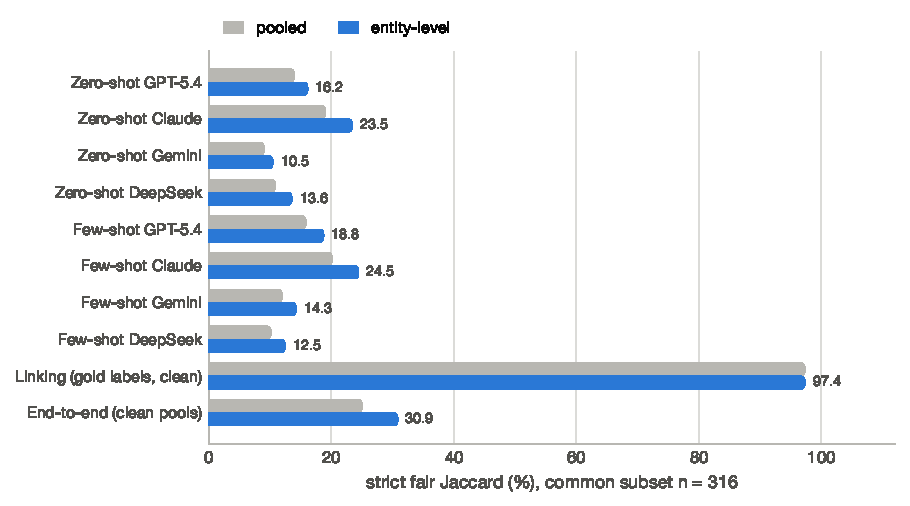
\includegraphics[width=0.88\textwidth]{figures/fig_main_comparison.pdf}
  \caption{Frozen models with and without the pipeline.}
  \label{fig:main}
  \tabnote{Strict fair set and common entity-defined subset.
The gold-label condition supplies the benchmark's query structure and is
used to isolate error sources; it is not presented as a performance
claim.}
\end{figure}

\subsection{Attributing the Error: Linking versus
Structure}

\label{sec:res-attribution}

For each question, the pipeline records whether it generated a query, whether all labels
were linked and whether the query executed.
\Cref{fig:funnel} shows these outcomes for the end-to-end
condition.

\begin{figure}[htbp]
  \centering
  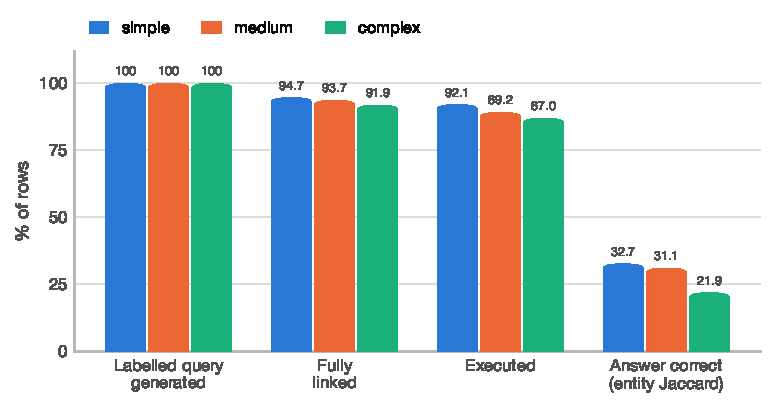
\includegraphics[width=0.88\textwidth]{figures/fig_stage_funnel.pdf}
  \caption{Stage-wise outcomes of the end-to-end pipeline, by query complexity.}
  \label{fig:funnel}
  \tabnote{Share of questions that pass each stage: labelled-query
generation, full linking, execution, and the final entity-level score.}
\end{figure}

Generation succeeds for 100\,\% of questions at every complexity level.
About 7\,\% of rows then lose a label during linking, and another 5\,\% fail to execute.
Final entity-level accuracy, over the 363 strict-set questions on which it is defined for this run, is 27.5\,\% and falls with complexity, from 32.7\,\% for simple questions to 21.9\,\% for complex ones.
On the common subset of 316 questions used to compare systems, the same run scores 30.9\,\% (\cref{tab:main}).

Most of the performance is lost at the final stage, but that alone does not isolate the cause.
Comparing the two conditions does.
On the common subset, given the benchmark's concepts and query structure, the pipeline reaches 97.4\,\%.
When it has to generate the query itself, it drops to 30.9\,\%, a difference of 66.5 points.
The gap therefore measures query generation, while disambiguation is measured directly in the linking comparison below.
The gap does not depend on the subset: on the full strict set of 400 questions, where a question without a scored query counts as zero, the two conditions reach 94.9 and 22.4 pooled Jaccard (\cref{tab:app-master}).

The gold-label condition is nearly tautological, because only the identifiers remain to be filled in, so it is not a performance result in itself.
Its value lies in the comparison between the two conditions.
The gap might suggest that structure explains all 66.5 points, but ``structure'' would then absorb every remaining source of error.
\Cref{fig:gap} breaks the gap down using the annotated failure sample.
Structural failures, that is the structure category together with the single triple flip (15 of 30 cases), make up 50.0\,\% of failing rows (95\,\% Wilson interval 33.2--66.8\,\%).
Applied to the 66.5-point gap, this share corresponds to 33.2 points.
Projection mismatches and residual identifier errors each account for about one fifth.
Structure is therefore the largest single component, especially for complex questions, while the rest of the gap comes from these other errors.
These figures are proportions of failing rows, not shares of the accuracy deficit, and they come from a 30-case sample (re-annotation agreement $\kappa$=0.62; agreement with an independent second annotator $\kappa$=0.595).

A second comparison changes only the candidate pools.
Building the pools with the rate-limited retrieval described in the method chapter raised gold-label accuracy by about 26 points, but end-to-end accuracy by only 2.6.
Better disambiguation thus helps a great deal when it is the only remaining task, and very little when the model also has to choose the concepts and build the structure.
This fits query generation being the main bottleneck.
The conclusion also does not rest on the annotated sample alone: the failure analysis examines construct use across all 567 reference queries and every generated run.

\begin{figure}[htbp]
  \centering
  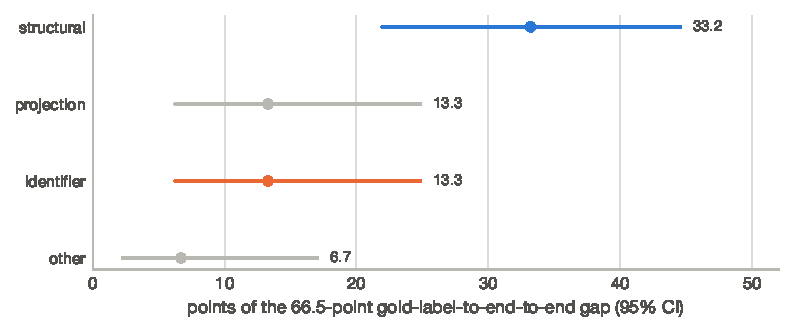
\includegraphics[width=0.88\textwidth]{figures/fig_gap_decomposition.pdf}
  \caption{What the 66.5-point gap is made of.}
  \label{fig:gap}
  \tabnote{Proportional attribution based on the 30-case taxonomy,
with Wilson intervals. The values are shares of failing rows, not of
the accuracy deficit.}
\end{figure}

\section{Linking Performance and Backbone
Dependence}

\subsection{Comparison of Linking
Paradigms}

\label{sec:res-linkers}

In the linking stage, every label in a query has to be mapped to the correct Wikidata identifier.
For each linker, precision, recall and F1 are computed at mention level against the ground truth derived from the benchmark: a prediction counts as correct only if it matches the reference identifier exactly, and a mention left unresolved counts against recall.

\begin{table}[htbp]
  \centering
  \caption{Entity and property linking across four paradigms, both splits.}
  \label{tab:linkers}
  \small
  \setlength{\tabcolsep}{3pt}
  \begin{tabular}{lllrrrr}
    \toprule
    Split & Linker & Backbone & Mentions & P (\%) & R (\%) & F1 (\%) \\
    \midrule
    working & Reasoning over candidates & Claude Opus 4.8 & entity & 97.8 & 97.6 & 97.7 \\
    working & Reasoning over candidates & Claude Opus 4.8 & property & 98.7 & 98.4 & 98.5 \\
    working & Reasoning over candidates & Qwen2.5-14B-Instruct & entity & 95.0 & 94.8 & 94.9 \\
    working & Reasoning over candidates & Qwen2.5-14B-Instruct & property & 98.0 & 97.7 & 97.9 \\
    working & Reasoning over candidates & Qwen2.5-7B-Instruct & entity & 95.8 & 95.7 & 95.8 \\
    working & GLiNKER gliner-linker-large-v1.0 & - & entity & 74.6 & 71.0 & 72.8 \\
    working & ELQ elq\_wiki\_large & - & entity & 67.1 & 18.0 & 28.4 \\
    working & ReFinED questions\_model & - & entity & 79.7 & 15.9 & 26.6 \\
    working & First search result & - & entity & 93.6 & 93.5 & 93.5 \\
    official & Reasoning over candidates & Qwen2.5-14B-Instruct & entity & 93.1 & 92.6 & 92.9 \\
    official & Reasoning over candidates & Qwen2.5-14B-Instruct & property & 97.8 & 97.0 & 97.4 \\
    official & GLiNKER gliner-linker-large-v1.0 & - & entity & 72.5 & 69.7 & 71.0 \\
    official & ELQ elq\_wiki\_large & - & entity & 71.7 & 22.1 & 33.8 \\
    official & ReFinED questions\_model & - & entity & 77.2 & 16.4 & 27.1 \\
    official & First search result & - & entity & 90.5 & 90.0 & 90.2 \\
    \bottomrule
  \end{tabular}
  \tabnote{Identical rows, identical ground truth and identical candidate pools within each split. P/R/F1 are mention-level; a prediction counts as correct only on exact identifier match. ELQ and ReFinED detect their own mentions, so their set-based figures are reported in the text instead. GLiNKER chooses among the same seven candidates per label as the reasoning linker. \emph{First search result} takes the first Wikidata search hit among those candidates, without any model, as a reference. Per-complexity F1 is plotted in Figure~\ref{fig:linker-cx} rather than repeated here.}
\end{table}


Four linking implementations were evaluated on the same rows, with the same ground truth, the same candidate pools where applicable, and the same scoring code.
The comparison is not fully symmetric: the reasoning-based linkers and GLiNKER choose from labels and curated candidates, whereas ELQ and ReFinED have to detect mentions in the question text themselves (see the limitations).
The paragraphs below assess how much of the ordering this difference explains.
\Cref{fig:linkers} shows entity-linking F1 on both splits, and~\cref{tab:linkers} gives the results.

\begin{figure}[htbp]
  \centering
  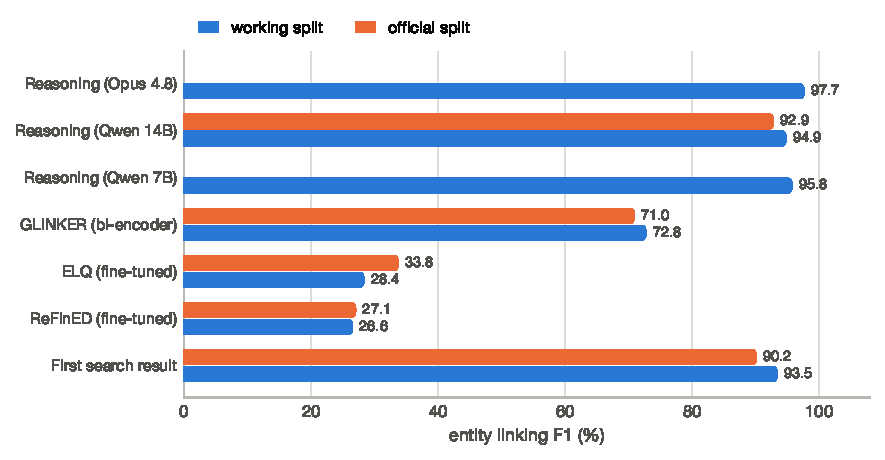
\includegraphics[width=0.88\textwidth]{figures/fig_linker_comparison.pdf}
  \caption{Entity linking F1 across four paradigms and two splits.}
  \label{fig:linkers}
  \tabnote{Within each split, all systems use identical rows,
ground truth and candidate pools. The first search result is a
reference without any model. On the official split, the reasoning
linker was run with the Qwen2.5-14B backbone only, which is available on
the group's GPU server; Claude Opus 4.8 (paid API) and Qwen2.5-7B were
evaluated on the working split.}
\end{figure}

With a frontier backbone, reasoning over retrieved candidates reaches 97.7 entity F1 and 98.5 property F1, and it resolves every identifier correctly in 89.9\,\% of queries.
The specialised linkers score lower: 72.8 (GLiNKER, choosing among the same candidates), 28.4 (ELQ) and 26.6 (ReFinED).
\Cref{fig:linker-ci} reports bootstrap confidence intervals for these scores, resampling the 1,086 entity mentions with replacement and applying the same resample to every linker in each draw.
The paired difference between the frontier reasoning linker and GLiNKER is 24.9 points $[22.3, 27.7]$, about five times the width of its own interval.
A reference point without any model shows where this accuracy comes from: taking the first Wikidata search result for each label reaches 93.5 on the working split and 90.2 on the official split.
Reasoning over the candidates adds 4.1 points $[2.7, 5.6]$ to it with the frontier backbone, 2.2 with Qwen2.5-7B and 1.4 with Qwen2.5-14B, the last within noise.
So most of the linking accuracy comes from labels that Wikidata's search can find, and the reasoning step resolves the remaining ambiguous cases, while GLiNKER's choice falls below the search order itself.
The intervals of the three reasoning backbones overlap, so they are not ranked against each other.
This similarity is the main finding of the backbone comparison below.

\paragraph{The Shape of the Deficit}

The specialised linkers' errors follow a clear pattern.
\Cref{fig:linker-pr} shows that ELQ and ReFinED, although developed independently, years apart and with different architectures, share a similar precision–recall profile (precision 67--80\,\%, recall 16--22\,\%): when they predict, they are usually right, but they do not predict often enough.
\Cref{fig:linker-cx} breaks F1 down by complexity: the two fine-tuned linkers are the only systems whose F1 falls as complexity rises (ReFinED 53.7$\to$35.6$\to$20.3; ELQ 34.1$\to$37.2$\to$23.3), while the linkers that choose among candidates hold steady or improve (frontier 92.9$\to$98.1$\to$97.7; GLiNKER 61.8$\to$70.7$\to$74.1).
This fits the mention-detection mismatch discussed earlier.
The set-based metric, which removes the mention-alignment penalty, lifts ELQ to 33.8 and ReFinED to 33.4 and so explains part, but not most, of the deficit.
ELQ's entity library, derived from Wikipedia in 2019, contains 72.4\,\% of the reference entities in the official split and 68.6\,\% in the working split.
So missing entities explain only a small part of a recall of 18--22\,\%, and mention detection most of it.

GLiNKER was evaluated outside the setting it was designed for, and ELQ and ReFinED solve a different sub-task because they detect their own mentions.
Neither issue, alone or combined, explains the ordering.
Given the same seven candidates as the reasoning linker, GLiNKER reaches 72.8 with candidate descriptions and 41.8 with labels alone, so the descriptions carry most of its gain.
The ordering holds on both splits: on the official split, GLiNKER reaches 71.0 against 92.9 for the reasoning linker with Qwen2.5-14B.

\paragraph{Replication on LC-QuAD 2.0}

Both splits come from the same dataset, so they cannot show whether the result carries over to other benchmarks.
Repeating the experiment on LC-QuAD 2.0 (gold-label condition; backbone, candidate depth, prompt and scoring held constant; 150 questions, 203 entity and 250 property mentions) gives 90.6\,\% entity accuracy $[85.8, 93.9]$ and 96.4\,\% property accuracy $[93.3, 98.1]$, with 96.7\,\% of queries fully linked.
The pattern found on Instruct-to-SPARQL reappears on a benchmark with different authors, templates and aims.

Entity accuracy is 4.3 points below the 94.9\,\% the same backbone reaches on Instruct-to-SPARQL, which lies outside the reported interval and cannot be explained by sampling noise alone (LC-QuAD 2.0 may contain more long-tail entities).
Unlike the labels in Instruct-to-SPARQL's annotated variant, its mention labels are the current Wikidata labels of the gold identifiers and are therefore findable by construction.
The reported value is an upper bound for this benchmark, and the comparison across benchmarks matters more than the absolute level.
This experiment replicates the linking measurement only.
The structural gap is measured on Instruct-to-SPARQL.
Separately, six of the 357 gold identifiers in the sample (1.7\,\%) no longer resolve against Wikidata, because they have been deleted or merged since the benchmark was published in 2019.

\subsection{Backbone Dependence by
Stage}

\label{sec:res-lcquad}

\label{sec:res-backbone}

The reasoning-based linker was evaluated again with two open-weight backbones, with the prompt, candidate pools, ground truth and evaluation procedure unchanged.
\Cref{fig:backbone} shows the results, which differ sharply between the disambiguation and label-generation stages.

\begin{figure}[htbp]
  \centering
  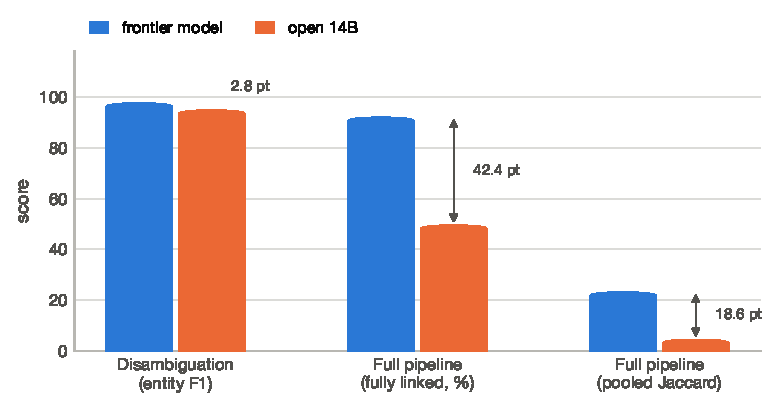
\includegraphics[width=0.88\textwidth]{figures/fig_backbone.pdf}
  \caption{Disambiguation and label-generation results by backbone.}
  \label{fig:backbone}
  \tabnote{Frontier model against the open 14B model: entity F1 at the
disambiguation stage (working split), and the fully linked rate and pooled
Jaccard of the official-split pipeline when the respective model generates
the labelled query.}
\end{figure}

At the disambiguation stage, the backbone makes little difference.
The frontier model reaches 97.7 entity F1, the 14-billion-parameter open model 94.9, and the 7-billion-parameter open model 95.8, with overlapping confidence intervals.

During label generation, the backbone matters more.
On the official split, using the open model for both stages drops the linked rate from 92.1\,\% to 49.7\,\%, and pooled accuracy from 23.4 to 4.8.

\Cref{fig:labelfail} shows why.
Asked to produce Wikidata entity and property labels on its own, the open model writes 270 of 1,645 distinct labels (16.4\,\%) that Wikidata's search index cannot find.
The frontier model writes 23 of 687 such labels (3.3\,\%) on the same questions.
The open model's failure rate is 4.9 times higher.

About half of the open model's unfindable labels are near-misses of existing property names, such as ``crew member(s)'' and ``is named after''.
Another 29\,\% are camelCase RDF-style identifiers, such as locatedInTheAdministrativeTerritory.
A further 3\,\% use snake\_case, and 2\,\% are bare property identifiers where a label was expected.
The frontier model produces none of these last three kinds.
The open model also generates 2.4 times as many distinct labels for the same questions, a sign of both lower consistency and lower accuracy.

\begin{figure}[htbp]
  \centering
  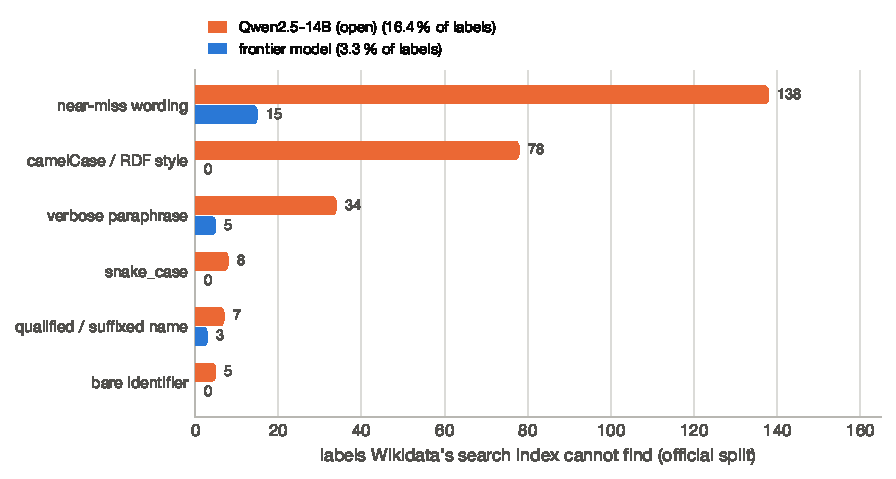
\includegraphics[width=0.88\textwidth]{figures/fig_label_failures.pdf}
  \caption{Unfindable labels by failure type and backbone.}
  \label{fig:labelfail}
  \tabnote{The figure includes labels that the Wikidata search index
cannot find. The official split is used, and labels are deduplicated
separately for both backbones. camelCase, snake\_case and bare
identifiers occur only for the open model and account for 34\,\% of its
unfindable labels.}
\end{figure}

One possible explanation is that the open model mainly has a formatting problem that a deterministic fix could solve.
This was tested with a normalisation procedure that splits camelCase, removes underscores, drops a leading ``is'' or ``has'', removes trailing parentheticals and singularises terms.
All 270 labels were normalised and searched again.

The procedure repaired 43 labels (15.9\,\%), lowering the failure rate from 16.4\,\% to 13.8\,\%.
Splitting camelCase recovered 36\,\% of the labels in that category, but such mechanical cases were only a minority of the failures.
The largest category could not be repaired, because terms such as ``significant achievement'' are alternative names for existing Wikidata properties.

The difference between the backbones at the generation stage is mainly a matter of knowing Wikidata's vocabulary.
Neither surface formatting nor reasoning ability explains it.
The next chapter discusses the practical implications.

\paragraph{Replication with Claude Opus 5}

All results so far use one frontier generator, so the diagnosis might reflect that particular model.
The baseline condition was therefore repeated with Claude Opus 5.
Nothing else changed: the system prompt, the absence of extended thinking, the disambiguation backbone and the scoring procedure stayed the same.

Accuracy rose from 27.03 to 32.66 entity-level Jaccard over 354 paired rows.
The construct counts show, however, that the improvement was uneven.

Compliance with subclass closure rose from 19.5\,\% to 43.6\,\%, and compliance with property paths from 13.4\,\% to 36.6\,\%.
Statement-node use increased from 18.5\,\% to 22.3\,\%, and qualifier use from 22.4\,\% to 28.2\,\%.
Value-node use did not improve at all: of the 35 reference queries that need a value node, both models use one in only two (5.7\,\%), and Opus 5 uses value nodes three times in total.

The newer model is much better at constructs that are mainly a matter of SPARQL syntax, and improves far less on constructs that require understanding how Wikidata represents information.
This mirrors the distinction drawn in the failure analysis below, between general-purpose SPARQL constructs, which models already use fairly often, and Wikidata-specific reification and hierarchy idioms, which remain difficult.

Opus 5 fully links 92.6\,\% of the 567 questions, against 95.2\,\% for Opus 4.8.
It produces six empty generations, where the earlier model produces none, and leaves 34 of 778 labels unresolved, against 25 of 852.
The candidate pool was pre-seeded and no rate limiting occurred, so these differences come from the backbone itself.
The newer model writes somewhat more labels that Wikidata's search index cannot find, which means its accuracy gain comes despite a slightly lower linking rate.

\section{Structural Failure
Analysis}

\label{sec:error-analysis}

The main failure pattern is characterised with evidence of increasing sample size: an annotated failure sample, construct counts across the corpus, and features of the reference queries.
The smallest is the easiest to interpret, and the largest gives the strongest evidence at corpus level.

\paragraph{Error Taxonomy}

\begin{table}[htbp]
  \centering
  \caption{Error taxonomy of a stratified sample of 30 failing questions.}
  \label{tab:errors}
  \small
  \resizebox{\ifdim\width>\textwidth\textwidth\else\width\fi}{!}{%
  \begin{tabular}{lrr}
    \toprule
    Category & n & Share (\%) \\
    \midrule
    structure & 14 & 46.7 \\
    near miss (projection) & 6 & 20.0 \\
    wrong property & 3 & 10.0 \\
    execution error & 2 & 6.7 \\
    unresolved label & 2 & 6.7 \\
    triple flip & 1 & 3.3 \\
    reference noise & 1 & 3.3 \\
    wrong entity & 1 & 3.3 \\
    \bottomrule
  \end{tabular}}
  \tabnote{Complexity-stratified random sample (seed 42) drawn from the reported clean-pool run and categorised by dominant error type. Each case was categorised by the author; an independent second annotator agreed on 21 of 30 cases. Proportions are indicative rather than population estimates.}
\end{table}


A complexity-stratified random sample of thirty failing questions was drawn from the reported end-to-end run, and each was classified by its dominant error type.
\Cref{fig:errors} and~\cref{tab:errors} show the distribution: structure accounts for 46.7\,\%, near misses for 20.0\,\%, wrong properties for 10.0\,\%, execution and unresolved errors for 6.7\,\% each, and triple flips, reference noise and wrong entities for 3.3\,\% each.
The gap attribution above groups the one triple flip with structure, because the query has the right properties but the wrong shape, which gives the structural group 15 of the 30 cases.

Structural errors are the largest category at every complexity level and are common among complex questions. Ten of the fifteen complex failures are structural.
Identifier-related errors still occur, though; three of the fifteen complex failures (20\,\%) come down to identifier selection.

The author categorised the cases in a single annotation pass, so the proportions describe recurring failure modes and should not be read as population-level frequencies.

\paragraph{Annotation Reliability}

To check the reliability of the categorisation, ten of the thirty cases were selected with an independent seed, anonymised and shuffled, and then re-annotated by the same person without access to the first classification.
Raw agreement was 7 of 10, and Cohen's $\kappa$ was 0.62, which is conventionally regarded as substantial agreement.

Two of the three disagreements concerned the boundary between structural and wrong-property errors, which is exactly the distinction the attribution analysis depends on.
Under the second annotation, the structural group fell from 15 to 14 of the 30 cases (50.0\,\% to 46.7\,\%), and the identifier-related share rose from 20.0\,\% to 26.7\,\%.
Structure stayed the largest single category, but by a smaller margin.

The second annotation also distinguished between an incorrect constraint, a missing constraint and missing aggregation.
The current taxonomy groups these cases under ``structure'', so the category is fairly broad.

\paragraph{A Second, Independent
Annotator}

Consistency within one annotator does not show that others read the categories the same way.
A second annotator, an undergraduate computer science student not involved in the project, classified all thirty cases independently, using only the written category guide, which is provided in the accompanying repository.

Raw agreement was 21 of 30, and Cohen's $\kappa$ was 0.595, slightly below the intra-annotator value.
The two annotators gave similar estimates for the category: the structure category accounted for 46.7\,\% of cases according to the author and 43.3\,\% according to the second annotator.
Only two of the nine disagreements concerned the boundary between structure and wrong-property errors.

The attribution therefore holds across two annotators.
Four of the nine disagreements, however, involved the quality of the reference query.
The second annotator pointed out specific issues: a missing country constraint, a missing class restriction, a grouped count where the question asked for items, and a flag that was computed but never used as a filter.
These judgements raise the estimated reference-noise rate in the sample from 3.3\,\% to 16.7\,\%.
Thirty rows cannot establish the true rate, so it is estimated on the full split below.

\paragraph{Bounding the Rate of Reference
Noise}

The full split was screened with five rules derived from the disputed cases (e.g.\ a superlative question whose reference query has no ordering or limit, or a nationality question whose reference has no country property), which flagged 61 of 400 strict-set queries (15.2\,\%).
A flag rate is not a noise rate, so a stratified sample of 40 flagged and 40 unflagged queries was adjudicated one by one (24 were dropped as unexecutable on the current snapshot, leaving 26 flagged and 30 unflagged).
Half of the flagged queries were judged faulty, against 6.7\,\% of the unflagged ones, which gives an initial estimate of 13.3\,\%.

A second independent judge, a doctoral student in computer science who was blind to the author's decisions and to the sampling strata, reviewed the same 56 rows.
Agreement was 73.2\,\% ($\kappa$=0.426).
The second judge's estimate was 32.0\,\%, against 13.3\,\% for the author.
The disagreement was systematic: 12 of the 15 cases went the same way, and they came from detection rather than from different standards of correctness. The author's first pass relied on the executed output, while the second judge also read the query text and caught issues such as a commented-out deduplication filter or an unchecked \texttt{OPTIONAL} block.

The two judges then reconciled the fifteen disagreements together against the query text and resolved ten in the second judge's favour.
The reconciled estimate is \textbf{24.6\,\% of the strict fair set, with an interval of $[12.9, 42.0]$}.
This counts the five cases that remained unresolved (genuine ambiguity about the intent of a loosely written question, not a checkable fact) as sound; counting them as faulty gives 32.0\,\%, the same as the second judge's independent estimate.
Reconciliation also showed that the screen's weakness is recall, not precision: its accuracy on the flagged group was unchanged (13/26 both before and after), while the fault rate in the unflagged group rose from 6.7\,\% to 20.0\,\%.

Roughly one quarter of the reference queries may therefore be unsound.
Some failures attributed to query structure may then come from the benchmark, and a system may be penalised for correctly answering a question that the benchmark encodes incorrectly.
The reported accuracy figures are not corrected for reference noise, for the comparability reasons discussed in the limitations.

\paragraph{Mechanism}

The structural failures follow a clear pattern: the model writes syntactically valid SPARQL but uses the direct-claim shortcut \texttt{wdt:} where the reference needs a more complex construct, such as transitive subclass closure, statement qualifiers, normalised value nodes, explicit aggregation, alternation, the lexeme model, or sitelink/badge access.
General-purpose SPARQL is handled well; the deficit is confined to Wikidata's reification and hierarchy idioms.
Averaging a height property directly instead of through its normalised value node, for example, silently mixes units and yields an arithmetically wrong result that the syntax alone does not reveal.
Near misses caused by projection mismatches, where the query returns a relation's object instead of its subject, were checked separately on ten additional zero-scoring rows.
All ten were indeed incorrect, so the reported accuracy needs no adjustment.
One further case in the sample was a reference query that did not answer its own question, an early sign of the reference-noise problem quantified above (24.6\,\% $[12.9, 42.0]$).

\paragraph{Corroboration across the
Corpus}

Because the sample is small, the same mechanism was tested at corpus scale across all 567 reference queries and every generated run (\Cref{fig:constructs}).

\begin{figure}[htbp]
  \centering
  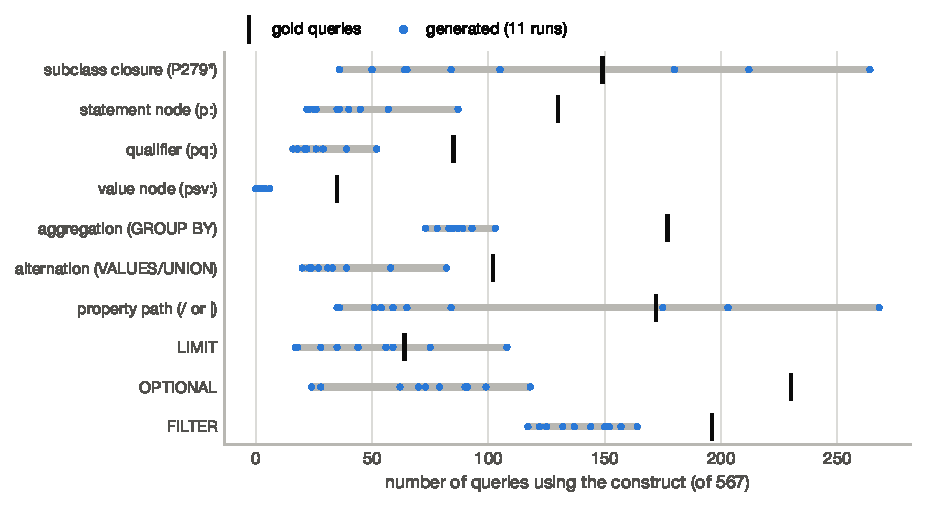
\includegraphics[width=0.88\textwidth]{figures/fig_constructs.pdf}
  \caption{Use of Wikidata's constructs: gold queries against all generated runs.}
  \label{fig:constructs}
  \tabnote{Each row shows the minimum and maximum count across the
eleven generated runs, while the rule indicates the count in the
reference queries.}
\end{figure}

Every system underuses Wikidata-specific constructs: of the 130 reference queries that use statement nodes, generated systems use them in 22--87; of 85 with qualifiers, in 16--52; and of 35 with normalised value nodes, in 0--4 (the strongest baseline never uses them).
General-purpose constructs (\texttt{FILTER}, \texttt{GROUP BY}, \texttt{OPTIONAL}) appear at rates close to the reference, so the deficit is specific to reification and hierarchy idioms, and it shows up across all four model families and both prompting regimes.

Usage counts alone cannot tell a system that never uses a construct from one that uses it in the wrong places, so~\Cref{fig:agreement} reports construct-agreement F1 instead.
Agreement is low and does not follow usage frequency: zero-shot GPT-5.4 uses subclass closure 212 times against 149 in the reference, yet agrees on only 54.8\,\% of questions, applying it where it is not needed and leaving it out where it is.
Only general-purpose constructs reach the 55--60 range.
So the models misplace these constructs as well as underusing them.

\begin{figure}[htbp]
  \centering
  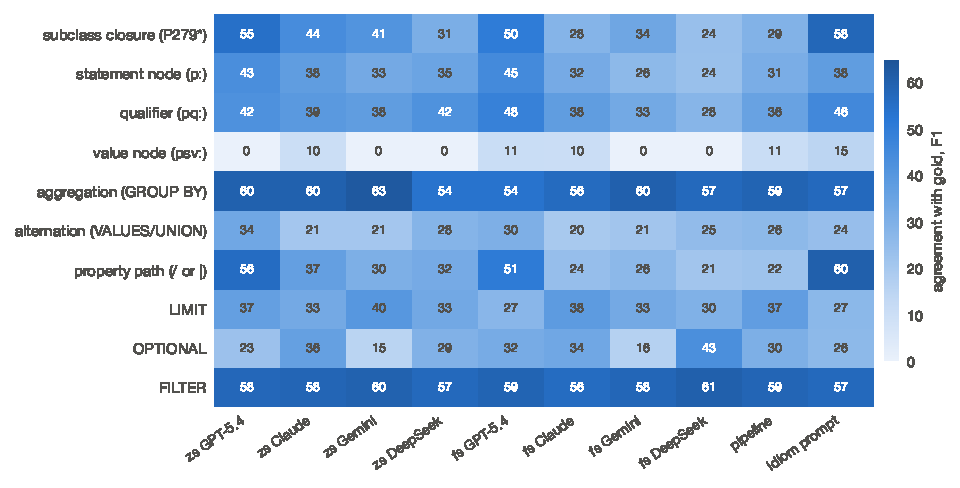
\includegraphics[width=0.88\textwidth]{figures/fig_construct_agreement.pdf}
  \caption{Agreement with gold on construct use, by system.}
  \label{fig:agreement}
  \tabnote{The figure reports per-question F1 for using a construct
exactly where it appears in the reference query. Usage counts alone
cannot distinguish missing use from excessive use, and agreement
measures both.}
\end{figure}

Finally, features of the reference query correlate with achieved accuracy in the expected direction (\cref{fig:predictors}): aggregation goes with 12.6 points lower accuracy, value nodes with 10.1, alternation with 9.6, transitive closure with 8.6 and statement nodes with 8.2, while \texttt{OPTIONAL} is the only feature linked to higher accuracy ($+10.9$).
These are weak differences in group means ($|\rho|\leq 0.15$), not predictive relationships.
They are reported because their ordering agrees with the taxonomy and the construct counts, so three independent measurements point in the same direction.
If this diagnosis is correct, telling the model explicitly about these constructs should help.

\section{Prompt Interventions and
Recovery}

\label{sec:res-noise}

\subsection{Prompt Interventions}

\label{sec:res-prompts}

\begin{table}[htbp]
  \centering
  \caption{Prompt interventions against the baseline arm: paired tests.}
  \label{tab:significance}
  \small
  \resizebox{\ifdim\width>\textwidth\textwidth\else\width\fi}{!}{%
  \begin{tabular}{lrrrrrr}
    \toprule
    Comparison & n & Mean difference (pp) & CI low & CI high & Permutation $p$ & Wilcoxon $p$ \\
    \midrule
    idiom guidance & 354 & 3.88 & 1.18 & 6.66 & 0.0054 & 0.0581 \\
    schema evidence, verbose & 336 & -14.65 & -18.94 & -10.38 & <0.001 & <0.001 \\
    schema evidence, targeted & 339 & -12.66 & -17.35 & -8.1 & <0.001 & <0.001 \\
    construct profile & 355 & 3.0 & 0.2 & 5.75 & 0.0342 & 0.0693 \\
    constrained vocabulary & 356 & 18.99 & 15.03 & 23.11 & <0.001 & <0.001 \\
    both oracles & 353 & 23.01 & 18.69 & 27.39 & <0.001 & <0.001 \\
    \bottomrule
  \end{tabular}}
  \tabnote{Paired over questions scored in both arms. Confidence intervals are bootstrap percentile intervals; the permutation test is two-sided. Only the generation prompt differs between arms.}
\end{table}


Seven generation conditions were compared, differing only in their system prompts.
\Cref{fig:arms} shows accuracy by intervention and the paired difference against the baseline, and~\cref{tab:significance} reports the statistical tests.
With a Holm correction for the six comparisons, every permutation result stays below 0.05.
The Wilcoxon signed-rank test, which uses the ranks rather than the sizes of the paired changes, is above 0.05 for idiom guidance (0.058) and the construct profile (0.069).

Idiom guidance gives a modest improvement.
Averaged over the questions each arm scored, entity-level accuracy rises from 26.8 to 30.2.
Over the 354 questions scored in both arms, the paired difference is $+3.88$ points $[1.18, 6.66]$, with a permutation result of $p = 0.005$.
The gain grows with query complexity, in line with the error analysis, where structural failures dominate at high complexity.

The average gain hides variation between questions, however.
Seventy questions improve, while 68 get worse.
The intervention shifts the overall level and distribution of performance, but it does not improve individual questions systematically.

Schema evidence has the opposite effect.
Averaged over the questions each arm scored, the verbose version lowers accuracy to 13.0 and the targeted version to 14.5.
The paired differences are $-14.65$ and $-12.66$, both with $p < 0.001$.
This runs against the improvements reported in research on schema-aware grounding, including~\parencite{zhang2026saga}.
The loss is about four times as large as the gain from idiom guidance.
It does not follow that retrieval augmentation is harmful in general: systems that combine retrieved context with an explicit validation or correction layer, rather than unconstrained prompt text, report gains from the same broad strategy~\parencite{pan2025firesparql}.
The finding here concerns schema evidence presented as evidence, not as a constraint.

\begin{figure}[htbp]
  \centering
  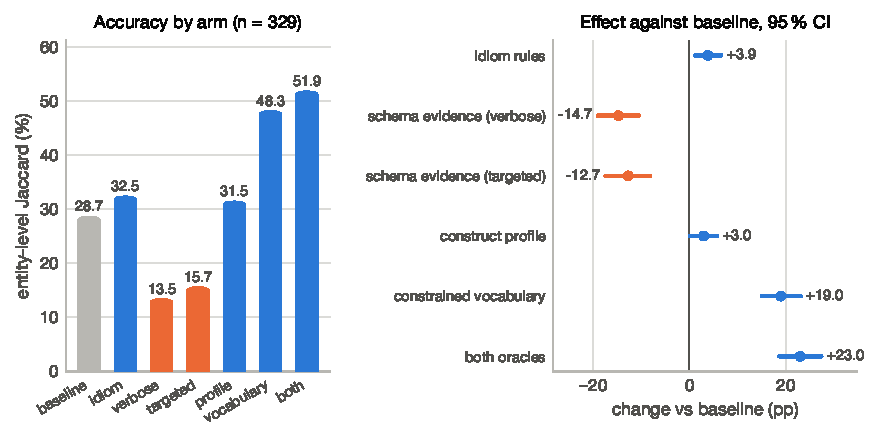
\includegraphics[width=0.88\textwidth]{figures/fig_prompt_arms.pdf}
  \caption{Prompt interventions: accuracy by arm and effect against the baseline.}
  \label{fig:arms}
  \tabnote{Only the generation prompt differs between conditions. The
generation model, candidate pools, disambiguation backbone and scoring
procedure remain constant. The left panel shows mean accuracy on the 329
rows scored in every arm. These levels are comparable across arms but
are slightly higher than the pairwise values in the text because the
latter use each comparison's own common rows. The right panel shows the
paired difference against the baseline with a 95\,\% bootstrap interval.}
\end{figure}

\paragraph{What the Interventions
Change}

\Cref{fig:idiom} shows how idiom guidance changes the generated queries: subclass closure rises from 50 to 264 (reference: 149), statement-node use from 25 to 45 (reference: 130), value-node use from 2 to 6 (reference: 35), and unrequested \texttt{LIMIT} clauses fall from 59 to 18.
Construct agreement improves most for the two constructs the prompt stresses most (subclass closure 29\,\%$\to$58\,\%, property paths 22\,\%$\to$60\,\%).
The prompt changes behaviour a lot, sometimes pushing simple syntactic constructs past the reference rate, but it does much less for constructs that require knowing how Wikidata represents information.
Value-node use barely moves, and aggregation does not change at all despite an explicit instruction to use it.

The construct counts suggest that over-application is the main way the grounding interventions fail: against reference counts of 149 subclass closures, 130 statement nodes and 85 qualifiers, the targeted schema arm produces 342, 256 and 142.
Shorter, conditional evidence increases over-application instead of reducing it.
The grounded arms also share only 38\,\% of their label vocabulary with the baseline, compared with 73\,\% for the idiom arm.
Schema evidence leads the model to rewrite its queries extensively, even though the schema cards were built from reference-linked mentions, a favourable setting in which the intervention fails.

\begin{figure}[htbp]
  \centering
  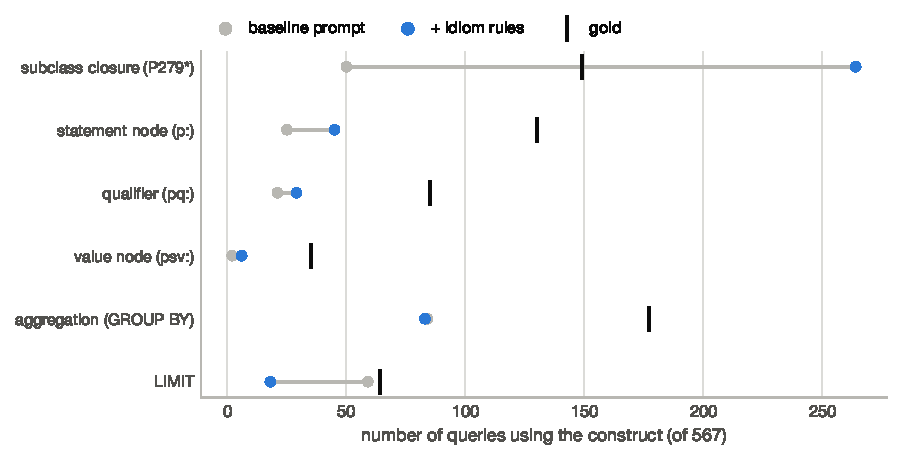
\includegraphics[width=0.88\textwidth]{figures/fig_idiom_behaviour.pdf}
  \caption{What the idiom prompt changes in the generated queries.}
  \label{fig:idiom}
  \tabnote{Number of the 567 generated queries that use each
construct under the baseline prompt and with the idiom rules. The
vertical mark gives the count in the reference queries.}
\end{figure}

\paragraph{Applying Guidance
Selectively}

If over-application is the problem, guidance could be given only when a query needs the relevant construct.
That requires two conditions, and the results fully support neither.
First, the need must be predictable from the question: a classifier that uses only the question text predicts construct use with an AUC of 0.62--0.82.
For subclass closure, its strongest features are topical terms (``libraries'', ``hospitals'', ``scientists''), because whether closure is needed depends on how Wikidata models the domain as well as on how the question is worded.
Second, guidance must do harm where it is not needed, and the results do not show this: idiom guidance helps most when the reference needs subclass closure ($+9.72$) or value nodes ($+7.97$), but it still raises accuracy by 2.0--4.3 points when no idiom is required.
On the 354 questions scored in both arms, an oracle gate that gives guidance only when a reification or hierarchy construct is present reaches 30.1, below the 31.2 of giving it unconditionally.
Selective application therefore does not beat always-on guidance, even with perfect knowledge of need, because over-application costs little.

\paragraph{Supplying the Knowledge
Directly}

If generic and selective guidance do not close the gap, the next question is what the model does when the missing knowledge is supplied directly.
Two interventions test two different kinds of information.

The construct-profile arm gives oracle information about which constructs the reference query uses, without revealing the query itself.
The model follows this information almost completely.
Subclass-closure compliance rises from 19.5\,\% to 100\,\%, and property-path compliance from 13.4\,\% to 95.3\,\%.
Compliance is lower for constructs that need more knowledge of how Wikidata stores facts, at 57.1\,\% and 61.2\,\%.

Despite this near-complete compliance, accuracy rises by only $+3.00$ points $[0.20, 5.75]$, no different from the gain from generic idiom guidance.
For the fourth research question, this means that the model can be told exactly which idiom is needed, and it will mostly use it, yet this adds little.
Knowing which construct is required is not the main bottleneck.

The constrained-vocabulary arm supplies a different kind of information.
It gives a closed list of the entities and properties that the reference query uses and forbids the model to use any identifier outside that list.
Accuracy rises by $+18.99$ points $[15.03, 23.11]$, with $p < 0.001$.
Here 141 questions improve and 41 get worse, which makes it the only intervention whose effect is consistently positive.

This is not a standalone performance claim: like the gold-label condition, the intervention receives part of the answer in advance, so its absolute performance is partly definitional.
The result is meaningful as a comparison, because the enumerative schema cards were built from the same reference-linked mentions.

The two arms receive information about the same entities and differ only in how it is presented.
Given as available evidence, it lowers accuracy by 14.65 points.
Given as a closed vocabulary that the model must use, it raises accuracy by 18.99 points.
The resulting difference of 34 points, with non-overlapping intervals, motivates the design principle discussed in the next chapter. Prompt-level intervention can still help, but more advice alone does not.

\paragraph{Which Knowledge Matters: A
Two-by-Two}

The two single-factor interventions supply different information and produce very different gains.
They correspond to the two generation decisions defined in the method chapter: the permitted vocabulary settles concept selection, and the construct profile names the idioms that structural composition needs.
A fourth arm, supplying both, completes a factorial design (percentile intervals from 10,000 bootstrap resamples) and shows that the effects are additive: construct information adds $+3.76$ points $[0.96, 6.58]$ even with the concepts fixed, and concept information adds $+19.72$ points $[15.30, 24.03]$ even when the required constructs are specified.
The jointly predicted result (21.99) matches the observed 23.01, and the one-point interaction lies within the intervals.
Concept selection thus accounts for the larger part of the error that these two oracles remove, and naming the idioms adds a smaller, independent part.
Neither oracle composes the query: with both supplied, entity-level accuracy reaches 50.4 on the 353 paired questions, whereas the gold-label condition, which supplies the composed query, reaches 97.4.
The model can recognise and use a named construct but still struggles to compose the correct query around the right concepts.

\paragraph{Type-Constraint Filtering}

The constrained-vocabulary arm restricts the generator through instructions, which it may ignore.
\citet{zhang2026saga} instead remove type-incompatible candidates mechanically before generation.
Filtering cannot be undone, so a removed candidate cannot be recovered by later reasoning.
The first thing to check is whether filtering keeps the correct property.
The test covers every property mention with at least two candidates including the reference property (1,132 mentions, 4.39 candidates on average).
A candidate is removed when it declares a Wikidata type constraint (P2302, constraint type Q21503250) and none of its permitted classes covers a subject type present in the question.
Subject types are taken from the row's reference entities via P31/P279 closure.
Of 1,062 candidate properties, 704 declare a type constraint.
Only 80 mark it as mandatory, while 616 have a type constraint without any status, so a violation is reported but not prohibited (a property can carry several such constraints).
Applying every declared constraint affects 79.8\,\% of mentions and shrinks the average pool from 4.39 to 3.02, but the reference property survives only 92.5\,\% of these operations.
Restricting the filter to mandatory constraints raises survival to 99.1\,\% but removes only about half a candidate per mention and resolves just three of the 1,132.

The two filters trade off differently: the stronger one removes the correct answer in roughly one of thirteen affected mentions, while the safer one removes almost nothing.
Even the safer estimate is generous.
The type universe combines all entity types in a row, subject types come from reference entities and not from a signal available at deployment, and forty-one mentions have no reference entity and would require abstention.

The principle of constraining rather than enumerating still holds, but implementing it mechanically is not straightforward.
Constraining the generator works when the constraint is correct.
A mechanical filter, however, is only as good as the quality and completeness of Wikidata's constraint declarations, and most of these are not marked as binding.

\subsection{Recovering Failures without Gold
Supervision}

\label{sec:res-filter}

\label{sec:res-cascade}

\begin{table}[htbp]
  \centering
  \caption{Selection strategies over diverse generations, entity-level Jaccard.}
  \label{tab:cascade}
  \small
  \resizebox{\ifdim\width>\textwidth\textwidth\else\width\fi}{!}{%
  \begin{tabular}{llrrr}
    \toprule
    Candidate pool & Selection & n & Entity-level Jaccard & Exact match (\%) \\
    \midrule
    one generator, three prompts & baseline arm & 349 & 26.3 & 8.3 \\
     & idiom arm & 349 & 30.2 & 11.5 \\
     & end-to-end run & 349 & 27.1 & 8.6 \\
     & cascade & 349 & 33.5 & 12.3 \\
     & centroid & 349 & 30.6 & 10.3 \\
     & centroid with fallback & 349 & 30.3 & 10.3 \\
     & oracle & 349 & 35.4 & 14.0 \\
    \midrule
    four zero-shot models & zero-shot Claude & 330 & 22.5 & 8.2 \\
     & zero-shot GPT-5.4 & 330 & 14.9 & 5.2 \\
     & zero-shot Gemini & 330 & 9.8 & 2.7 \\
     & zero-shot DeepSeek & 330 & 12.3 & 3.9 \\
     & cascade & 330 & 23.7 & 8.2 \\
     & centroid & 330 & 24.5 & 8.5 \\
     & centroid with fallback & 330 & 24.2 & 8.5 \\
     & oracle & 330 & 28.0 & 10.9 \\
    \midrule
    all eight runs & idiom arm & 327 & 32.2 & 12.2 \\
     & end-to-end run & 327 & 29.0 & 9.2 \\
     & baseline arm & 327 & 28.1 & 8.9 \\
     & few-shot Claude & 327 & 23.4 & 7.3 \\
     & zero-shot Claude & 327 & 22.6 & 8.3 \\
     & zero-shot GPT-5.4 & 327 & 15.1 & 5.2 \\
     & zero-shot DeepSeek & 327 & 12.5 & 4.0 \\
     & zero-shot Gemini & 327 & 9.8 & 2.8 \\
     & cascade & 327 & 37.0 & 13.5 \\
     & centroid & 327 & 33.8 & 10.7 \\
     & centroid with fallback & 327 & 34.1 & 11.0 \\
     & oracle & 327 & 44.1 & 19.0 \\
    \bottomrule
  \end{tabular}}
  \tabnote{Each selector uses only the candidates' own result sets, never the gold answer. \emph{oracle} is the best candidate per question and is an upper bound, not a system. Figures come from a re-execution of the cached queries and sit 0.8--1.4 points below the scores elsewhere in the results; they are internally consistent and should not be mixed with those tables.}
\end{table}


The interventions above change the queries the model generates.
This section asks instead whether the correct query can be picked from several candidates without looking at the reference query.
As shown earlier, an empty result is always wrong in this evaluation, and empty results are common, so execution validity is a signal available at inference time.
\Cref{fig:cascade} and~\cref{tab:cascade} compare selection strategies across the existing runs.

An oracle that picks the best query from the eight available runs reaches 44.1 entity-level Jaccard, against 32.2 for the best individual run, a gap of about twelve points.
The question is how much of this a practical selector can recover.

The cascade accepts the first query, in a fixed order, that returns a non-empty and error-free result.
It reaches 37.0 Jaccard, against 32.2 for the best single run.
This is a gain of +4.83 points [2.93, 7.08], with a permutation-test result of p \textless{} 0.0001.
The selection changes the output for 49 questions, and all 49 changes improve the score.
This follows from how the cascade is built: it only replaces results that score zero to begin with.
A split-half evaluation, which chooses the order on one half of the questions and evaluates it on the other, reproduces the gain out of sample at +5.4 and +4.3.

\Cref{fig:fallback} shows where the fallback is applied.
It is triggered for 92 of 327 questions (28\,\%), and in 64 of these the preferred query returns no results.
Since an empty result scores zero by construction, the cascade recovers 16.3 Jaccard points on these questions.
The improvement is fairly even across complexity levels, unlike that of the idiom prompt, whose benefits concentrate on the more complex questions.

\begin{figure}[htbp]
  \centering
  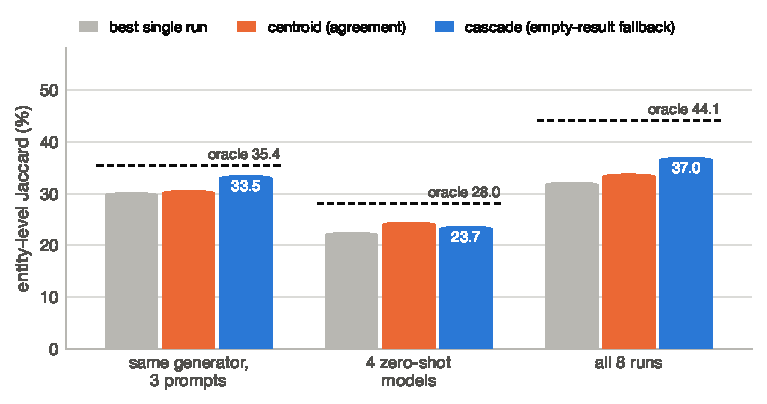
\includegraphics[width=0.88\textwidth]{figures/fig_cascade.pdf}
  \caption{Selection strategies over diverse generations.}
  \label{fig:cascade}
  \tabnote{Entity-level Jaccard. The dashed line represents the
oracle, which is an upper bound rather than an executable system. The
figures are based on the separate execution pass described in
this section and should not be directly compared with the
other tables in this chapter.}
\end{figure}

Selection by agreement does only slightly better than the individual runs: the result-set centroid reaches 33.8, against 37.0 for the cascade.
That does not mean agreement carries no useful information.
Candidates whose result sets agree with another candidate at 0.9 or above reach an average entity-level Jaccard of 43.8 against the reference, while candidates that agree with no other candidate reach only 13.3.

This information is largely redundant, however.
When several candidates agree, the preferred run is usually already among them.
When they disagree, the centroid often picks a plausible majority rather than the correct minority.
Where most candidates are wrong, checking whether the preferred query is valid is more useful than voting among all of them.

The results in this section come from a separate execution pass.
Its single-run scores are 0.8 to 1.4 points lower than the corresponding scores elsewhere in the chapter, because of endpoint state and the cap on returned values.
The comparisons within this section are internally consistent, but these figures should not be combined with the other tables.
The cascade order also uses knowledge of how good the runs are relative to each other.
The split-half analysis shows that the gain holds out of sample, but a deployed system would have to choose the order on a validation split.

\section{Benchmark Comparison and
Validity}

\subsection{Comparison with the Benchmark Authors'
Systems}

\label{sec:res-authors}

The benchmark authors publish generated queries for every test question under fourteen configurations.
Re-executing these stored outputs on the dump used here, with the same fair set and evaluation metric, allows a comparison free of additional inference variation, as shown in~\Cref{fig:frozen}.

\begin{figure}[htbp]
  \centering
  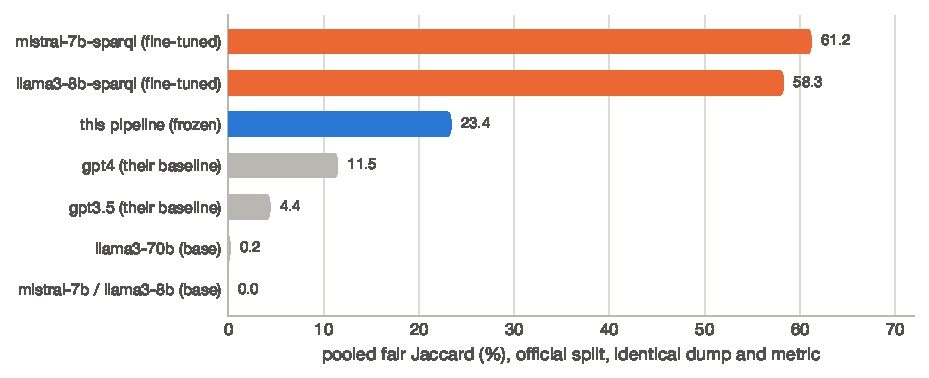
\includegraphics[width=0.88\textwidth]{figures/fig_frozen_vs_finetuned.pdf}
  \caption{Frozen and fine-tuned systems on the official split.}
  \label{fig:frozen}

\end{figure}

\emph{Figure note}.
All systems are evaluated on the same dump using the same strict fair set and metric.
The authors' results come from re-executing their published generated queries.

Every system is scored on all 370 strict-set questions of the official split, and a question for which a system produced no query counts as zero.
The fine-tuned models reach pooled fair Jaccard scores of 61.2 and 58.3, and the pipeline developed here reaches 23.4.
The authors' GPT-4 and GPT-3.5 baselines reach 11.5 and 4.4, respectively.
Without any in-domain training, the pipeline more than doubles the authors' frozen baselines and reaches more than one third of the fine-tuned systems' score.
Since its disambiguation is near-perfect, the remaining difference once more points to query generation.
This is a comparison between systems: the pipeline also uses a newer generator than the authors' GPT-4 baseline.
The pipeline's own contribution is measured on the working split, where it adds 6.0 pooled points over the same generator used zero-shot (19.1 to 25.1, \cref{tab:main}).

Of the best fine-tuned model's outputs, 56\,\% are character-identical to the reference query.
By contrast, exact and identifier-masked overlap between training and test queries is only 0.6\,\%, and the authors' training code loads the official training split.
This does not establish data leakage.
It rather suggests that fine-tuning teaches the model to reproduce the highly templated query style of the benchmark.
The benchmark was crawled from tutorial pages, and fine-tuning on 1,854 in-distribution queries exposes the model directly to this style.
A structural memorisation test indicates that the advantage extends beyond direct recall: accuracy is 55.1\,\% for rows whose structure closely matches a training query and 52.5\,\% for rows without such a match.

Base models without fine-tuning score at or near zero.
Llama 3 70B, for example, reaches only 0.2\,\% accuracy, with an execution rate of 14.2\,\%.
On this benchmark, the fine-tuned 7B model is roughly three hundred times more accurate than the base 70B model.
Model scale alone, it seems, does not replace what fine-tuning contributes.
One possible explanation is that fine-tuning improves conformity to the expected query idiom, the same capability that this chapter found lacking in the frozen models.

\subsection{Validity Checks}

\label{sec:res-validity}

\paragraph{Memorisation Check}

\begin{table}[htbp]
  \centering
  \caption{Structural similarity of generated queries to the benchmark.}
  \label{tab:memorisation}
  \small
  \resizebox{\ifdim\width>\textwidth\textwidth\else\width\fi}{!}{%
  \begin{tabular}{lrrrrrrrrrr}
    \toprule
    Run & n & Identical & $\geq$0.95 & $\geq$0.90 & Other, mean & Other $\geq$0.90 & Acc.\ close & Acc.\ other & n close & n other \\
    \midrule
    Zero-shot GPT-5.4 & 400 & 0.0 & 1.5 & 6.8 & 0.879 & 57.8 & 18.4 & 9.1 & 210 & 140 \\
    Zero-shot Claude & 400 & 0.0 & 1.2 & 7.5 & 0.9 & 66.0 & 23.2 & 18.0 & 249 & 106 \\
    Zero-shot Gemini & 400 & 0.2 & 2.2 & 11.2 & 0.91 & 67.8 & 10.8 & 7.6 & 238 & 104 \\
    Zero-shot DeepSeek & 398 & 0.0 & 1.0 & 6.8 & 0.847 & 47.5 & 13.5 & 11.6 & 170 & 174 \\
    Few-shot Claude & 400 & 0.0 & 2.2 & 9.8 & 0.918 & 74.2 & 24.7 & 14.5 & 276 & 81 \\
    End-to-end pipeline & 400 & 0.0 & 3.2 & 10.2 & 0.905 & 69.2 & 29.8 & 21.6 & 262 & 101 \\
    Idiom arm & 397 & 0.0 & 1.3 & 7.8 & 0.883 & 58.2 & 35.8 & 21.2 & 225 & 140 \\
    \bottomrule
  \end{tabular}}
  \tabnote{Skeletons compare query shape only: identifiers, literals, variable names, numbers and prefixes are removed. \emph{Identical} is the memorisation test; \emph{Other} measures resemblance to any other dataset query and reflects genericness rather than recall. For reference, 56\% of the benchmark authors' fine-tuned model's outputs are character-identical to the reference query. \emph{Identical}, $\geq$0.95 and $\geq$0.90 give the share of outputs (\%) whose skeleton is identical or that similar to its own reference; \emph{Other} is the best similarity to any other dataset query (mean, and share $\geq$0.90 in \%); \emph{Acc.} is entity-level Jaccard on rows whose structure is close ($\geq$0.90) to another dataset query and on the other rows.}
\end{table}


The Instruct-to-SPARQL dataset has been public since May 2025, while the models evaluated here were released in 2026 and their training data are undisclosed.
Memorisation is a real concern.
Recent work on LLM-generated SPARQL likewise shows that memorisation and externally injected graph knowledge can substantially affect apparent benchmark performance, which makes a direct check necessary~\citep{gashkov2025memorization}.
The check uses the same skeleton comparison as the earlier analysis: identifiers, literals, variable names, numbers and prefixes are removed, leaving only the query structure.

No frozen run reproduces the reference structures to any substantial degree.
Between 0.0\,\% and 0.2\,\% of outputs are skeleton-identical to their own reference query, and 1.0\,\% to 3.2\,\% reach a similarity of at least 0.95.
This contrasts with the 56\,\% of character-identical outputs reported for the benchmark authors' fine-tuned model.
\Cref{fig:memorisation} and~\cref{tab:memorisation} report the distributions.

The figure also includes a measure that could be mistaken for evidence of copying.
Between 47.5\,\% and 74.2\,\% of generated skeletons have at least 0.90 similarity to some other query in the dataset.
This does not necessarily indicate memorisation.
Generated skeletons are often simple, and simple structures naturally resemble many other queries.
The rate is also higher than the 36.5\,\% similarity rate among the reference queries themselves.

Structural simplicity likewise explains the apparent accuracy advantage on questions that are structurally close to known queries.
Within complexity groups, the difference shrinks or disappears: zero-shot Claude, for example, scores 23 versus 22 on medium questions and 19 versus 16 on complex ones.
The test detects structural reproduction, not memorisation of a complete mapping from question to answer.

\paragraph{Representativeness of the Benchmark}

\begin{table}[htbp]
  \centering
  \caption{Construct prevalence: benchmark gold queries versus real query logs.}
  \label{tab:wdql}
  \small
  \resizebox{\ifdim\width>\textwidth\textwidth\else\width\fi}{!}{%
  \begin{tabular}{llrr}
    \toprule
    Queries & Construct & Benchmark (\%) & WDQL (\%) \\
    \midrule
    all & subclass closure (P279*) & 23.6 & 12.8 \\
     & statement node (p:) & 23.1 & 6.7 \\
     & qualifier (pq:) & 15.1 & 3.8 \\
     & value node (psv:/psn:) & 6.1 & 0.8 \\
     & aggregation (GROUP BY) & 31.9 & 11.5 \\
     & alternation (VALUES/UNION) & 17.3 & 12.8 \\
     & property path (/ | * +) & 38.8 & 16.8 \\
     & OPTIONAL & 39.9 & 29.8 \\
     & FILTER & 36.2 & 59.6 \\
     & LIMIT & 10.8 & 26.0 \\
     & any reification or hierarchy idiom & 41.2 & 18.8 \\
    \midrule
    5+ predicate tokens & subclass closure (P279*) & 31.6 & 25.6 \\
     & statement node (p:) & 37.4 & 18.9 \\
     & qualifier (pq:) & 24.7 & 13.1 \\
     & value node (psv:/psn:) & 11.3 & 3.3 \\
     & aggregation (GROUP BY) & 33.6 & 15.7 \\
     & alternation (VALUES/UNION) & 24.8 & 21.8 \\
     & property path (/ | * +) & 53.6 & 34.9 \\
     & OPTIONAL & 53.6 & 53.9 \\
     & FILTER & 46.9 & 83.6 \\
     & LIMIT & 10.3 & 33.7 \\
     & any reification or hierarchy idiom & 58.8 & 41.2 \\
    \bottomrule
  \end{tabular}}
  \tabnote{WDQL is the Wikidata Query Logs dataset (one-per-cluster release, 226{,}376 real queries). Size bands are predicate-token counts, a formatting-robust proxy for triple patterns. Counts: 2{,}838 benchmark and 226{,}376 WDQL queries in all; 1{,}525 and 51{,}728 with 5+ predicate tokens.}
\end{table}


The main findings concern query constructs measured on a benchmark collected from tutorial pages.
Whether these constructs also matter in everyday Wikidata use is a separate question.
To answer it, the benchmark is compared with the Wikidata Query Logs dataset~\parencite{walter2026wdql}, which contains 226,376 real queries sent to the public query service.

Across all queries, the benchmark contains substantially more reification and hierarchy idioms.
At least one such construct appears in 41.2\,\% of benchmark reference queries, against 18.8\,\% of query-log queries (\cref{fig:wdql}).
Benchmark queries are, however, generally larger, so query size affects this comparison.

When both datasets are restricted to queries with at least five predicate tokens (\cref{fig:wdql-size}), the difference shrinks but remains visible:

\begin{itemize}
\item
Any reification or hierarchy idiom: 58.8\,\% versus 41.2\,\%
\item
Subclass closure: 31.6\,\% versus 25.6\,\%
\item
Statement nodes: 37.4\,\% versus 18.9\,\%
\item
Value nodes: 11.3\,\% versus 3.3\,\%
\end{itemize}

\begin{figure}[htbp]
  \centering
  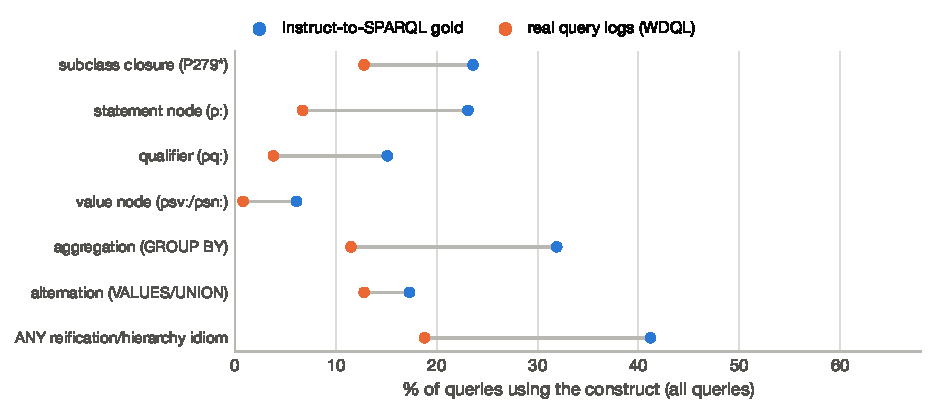
\includegraphics[width=0.88\textwidth]{figures/fig_wdql.pdf}
  \caption{Construct prevalence: benchmark gold queries against real Wikidata query logs.}
  \label{fig:wdql}
  \tabnote{The comparison includes all queries in both datasets.
Benchmark queries are larger on average, which confounds the comparison.
\cref{fig:wdql-size} controls for query size.}
\end{figure}

The relevant idioms are not just artefacts of the benchmark: roughly two in five non-trivial queries use at least one of them, so a system that cannot generate them will fail on a substantial share of real Wikidata queries.
The benchmark does, however, over-represent these constructs.
At matched query sizes, they are about 1.2 to 2 times more frequent in the benchmark, and value nodes around 3.4 times.
The accuracy reported here may therefore underestimate performance on questions distributed more like real query logs.

The comparison has limits of its own.
The query-log questions were generated by a model.
The logs also date from 2017--2018 and include bot traffic, which may explain the relatively high frequency of FILTER and LIMIT clauses.
